\section{Introduction}

Dialogue system is an important interface between machine and human.  An intelligent dialogue agent is not only required to give the appropriate response based on the current utterance from the user, but also consider the dialogue history. Dialogue context modeling has been a key point for developing such dialogue systems, including researches on state tracking~\cite{abs-1907-01669,RenNM19}, topic segmentation~\cite{NanDNX19,kim2019dynamic}, multi-turn response selection~\cite{TaoWXHZY19,GuLL19}, next utterance generation~\cite{abs-1911-00536,ChenCQYW19}, etc. In this paper, we target on the multi-turn response selection task, which is first proposed by Lowe et al.~\shortcite{LowePSP15} and is also a track in both DSTC7~\cite{gunasekara2019dstc7} and DSTC8~\cite{dstc8}.


Given a dialogue history made up of more than one utterance, the selection task is to choose the most possible next utterance from a set of candidate responses.  Previous work on this task can be roughly divided into two categories: sequential models and hierarchical models. The former ones, including \cite{LowePSP15,YanSW16,abs-1901-02609}, concatenate the history utterances into a long sequence, try to capture the similarities between this sequence and the response and give a matching score. The latter ones, including \cite{TaoWXHZY19,WangWC19,GuLL19}, extract similarities between each history utterance and the response first. Then, the matching information is aggregated from each pair 
(mostly in a chronological way) to get a final score. 
There is little difference between the performance of these two kinds of 
architectures until the emergence of large pre-trained language models.
 
 \begin{figure}
 	\centering
 	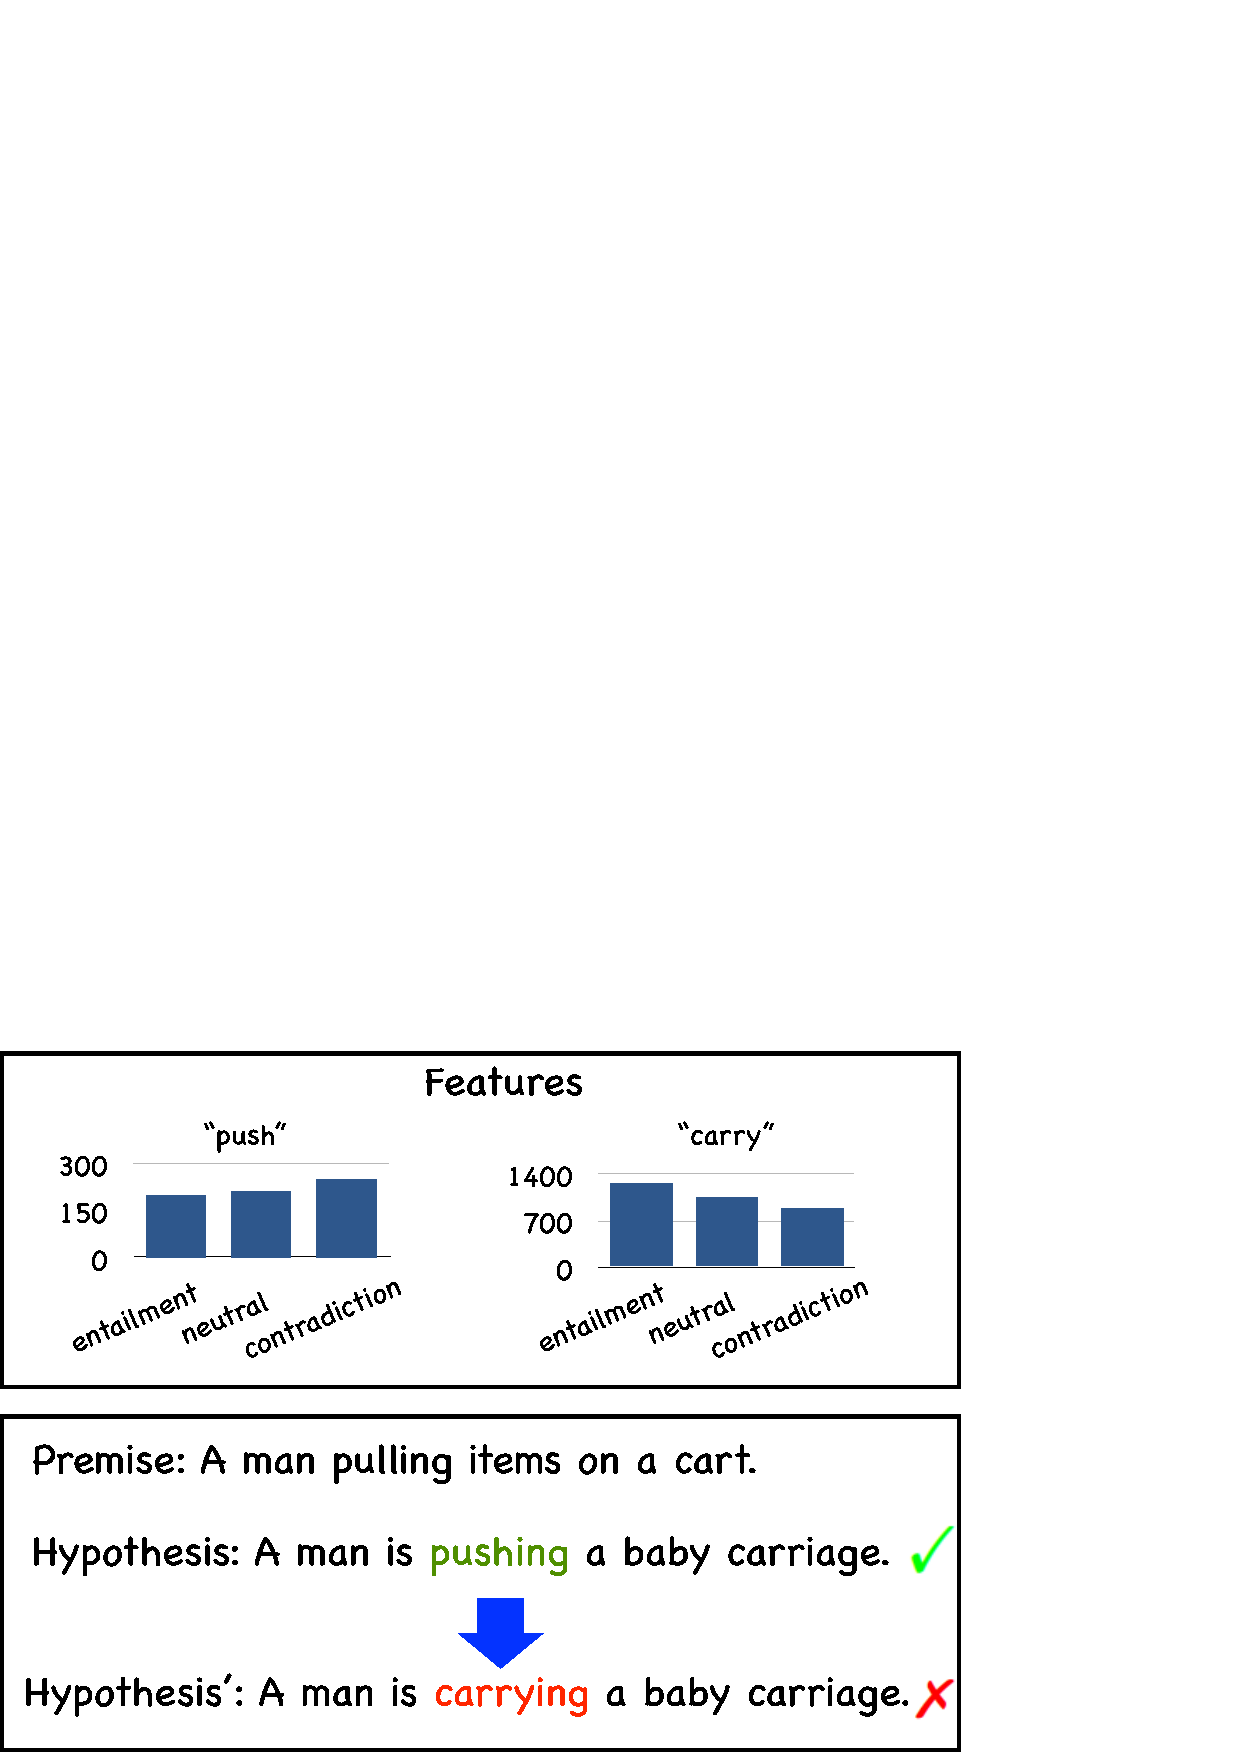
\includegraphics[scale=0.39]{pic/example.pdf}
 	\caption{An example of the tangled dialogue history. A, B and C are three participants. Texts in different colors represent different dialogue threads.}
 	\label{fig:example}
 \end{figure}
 
 
Work such as \cite{abs-1908-04812,vig2019comparison} has shown the 
extraordinary performance of the pre-trained language models on dialogues. 
These pre-trained models are easily transferred to the response selection 
task by concatenating all of the utterances as the input. 
All of the words in dialogue history can directly interact with each other 
via transformers like Bi-encoder, even the words both in the dialogue history 
and the candidate response if time permits, such as Cross-encoder~\cite{humeau2019poly}. 
However, since such models can be regarded as the ultimate 
architecture of the sequential-based models, the dialogue dependency 
information between the utterances is largely ignored due to the 
concatenation operation~\cite{WuWXZL17}. An example is shown in Figure \ref{fig:example}. The dependency relations can definitely help us to understand the two tangled dialogue threads.
Besides, we always need to truncate the earlier dialogue history 
to limit the size of the model and make the computation efficient. 
However, it isn't always that the nearest utterances are more important. 
As we can see in Figure \ref{fig:example}, several dialogue threads may 
be tangled especially in multi-party chat rooms, 
it's hard to tell which dialogue thread will be moving on.

In this paper, we propose to incorporate dialogue dependency information 
into the response selection task. 
We train a dialogue dependency parser
to find the most probable parent utterance for each utterance in a session. We name such relation between utterances as ``reply-to''.
Then, we empirically design an algorithm to extract dialogue threads, which is represented by a path of dependency relations according to the parsed trees.
The extracted threads are sorted by the distance between the final utterance in each 
thread and the response in ascending order, following the intuition that the closer utterances are more relevant.
After that, we propose the model named Thread-Encoder based on a pre-trained language 
model.
Each encoder in the model can distill the critical information from each dialogue thread or the candidate response. 
Finally, another attention layer is used to calculate the matching score 
with thread representations and the candidate representation. The candidate with the highest matching score will be selected as the final response.

We collect the training data for dialogue dependency parser from a dialogue 
disentanglement dataset~\cite{KummerfeldGPAGG19} in the technical domain. 
And we do response selection experiments among UbuntuV2, DSTC7 and DSTC8*. 
These datasets consist of dialogues in the same domain but under different settings, 
including two-party dialogues and multi-party dialogues. 
The results demonstrate our model's strong capability to represent multi-turn
dialogues on all of these datasets.

 
Our main contributions are as follows:
\begin{itemize}
	\item As far as we know, we are the first to incorporate dialogue 
dependency information into response selection task, 
demonstrating that the dependency relations in the dialogue history 
are useful in predicting dialogue responses (Sec \ref{sec:relatedwork}). 
	\item Based on the predicted dependencies, we design a straight-forward but effective algorithm to extract several threads from the dialogue history  (Sec \ref{sec:DSA}). 
The results show the algorithm is better than other simple segmentation 
methods on the response selection task.
	\item We propose the Thread-Encoder model, incorporating dialogue 
dependency information by threads and utilizing the pre-trained language 
model to generate corresponding representations (Sec \ref{sec:tem}). The experimental results 
show that our model outperforms the state-of-the-art baselines on 
DSTC7 and DSTC8* datasets, and is very competitive on UbuntuV2 (Sec \ref{sec:ra}).
\end{itemize}





